% f=triage; latex $f.tex; bibtex $f; latex $f.tex; latex $f.tex; dvips -t letter $f; ps2pdf $f.ps; evince $f.pdf
%% bare_conf.tex

\documentclass[conference]{IEEEtran}
\usepackage{verbatim}
%\usepackage{multirow}
\usepackage{array}
\usepackage{balance}
\usepackage{epsfig}
\usepackage{eqparbox}
\usepackage{url}
\usepackage{verbatim}
\usepackage{stfloats}
\usepackage{epstopdf}
%\usepackage{cite}
\usepackage[center]{caption}

\IEEEoverridecommandlockouts

\newtheorem{observation}{\bf Observation}

\hyphenation{op-tical net-works semi-conduc-tor}


\begin{document}

\title{Impact of Triage: a Study of Mozilla and Gnome}
%quantifying triage actions in bugzilla and gnome

\author{\IEEEauthorblockN{Jialiang Xie\IEEEauthorrefmark{1},
Minghui Zhou\thanks{*Corresponding author}\IEEEauthorrefmark{1} and
Audris Mockus\IEEEauthorrefmark{2}
}
\IEEEauthorblockA{\IEEEauthorrefmark{1}School of Electronics Engineering and Computer Science, Peking University\\
Key Laboratory of High Confidence Software Technologies, Ministry of Education\\
Beijing 100871, China\\
\{xiejl11@sei.,zhmh@\}pku.edu.cn}
\IEEEauthorblockA{\IEEEauthorrefmark{2}
Avaya Labs Research\\
233 Mt Airy Rd, Basking Ridge, NJ\\
audris@avaya.com}
}

\maketitle

\begin{abstract}
  Triage is of great interest in software projects because it has
  the potential to reduce developer effort by involving a broader
  base of non-developer contributors to filter and augment reported
  issues.  Using issue tracking data and interviews with
  experienced contributors we investigate ways to quantify the
  impact of triagers on reducing the number of
  issues developers need to resolve in two OSS projects:
  Mozilla and Gnome. We find the primary impact of triagers to
  involve issue filtering, filling missing information, and
  determining the relevant product. While triagers were good at
  filtering invalid issues and as accurate as developers in filling
  in missing issue attributes, they had more difficulty accurately
  pinpointing the relevant product. We expect that this work will
  highlight the importance of issue triage in software
  projects and will help design further studies on understanding and
  improving triage practices.
\end{abstract}

\IEEEpeerreviewmaketitle

\section{Introduction}
%the motivation is to do a more in--depth study to understand triage and its impact
Developing source code is not enough for a successful software
project. Necessary levels of quality and completeness of
functionality could be realized only through feedback from a large
population of contributors, especially users. Such input is typically
managed via issue tracking systems (ITS).  A small core team~\cite{MFH02}
of popular OSS projects can be easily overwhelmed by the massive inflow
of issues ($>50$K/year in Mozilla and Gnome) leading to
delays, unsatisfied users, and lower quality of the product.
In particular, a considerable number of reported issues are of low
quality and can not be fixed. For example, issues lacking sufficient
information represent 15\% and 6\% of all resolved issues in Gnome and
Mozilla~\cite{MM12}. It is, thus, paramount to
recruit, train, and retain a broader base of contributors (triagers)
to filter and augment this predominantly low-quality input, so that
the developers can spend their time on fixing real issues. Triage as
a procedure to filter and improve the quality (relevance, accuracy,
reproducibility, non-duplication, and completeness) of user reported
issues is, thus, a critical part of any large project.
% because unlike a
%smaller group of testers, it is impossible and impractical to train
%{\em all} users to report only high-quality issues.

%A considerable number of reported issues are of low quality and can
%not be fixed. For example, issues lacking sufficient information
%represent 15\% and 6\% of all resolved issues in Gnome and
%Mozilla~\cite{MM12}.  Attempts to reproduce such issues would take
%time away and delay or prevent fixing of real defects and,
%therefore, may affect product quality and lead to bad user
%experience.

Many contributors help with issue reporting and resolution.  For
example, Gnome project Evolution had more than $20$K contributors
helping to report and resolve issues, but only 1K developers
contributing code over the past decade. However, the value of
contributions made by these non-developer triagers may be
underestimated. A developer who does a triage on an issue, can also
fix the issue, unlike the non-developer triagers. Consequently,
non-developer triagers may feel unappreciated, e.g., a triager left
Mozilla ``because of a general lack of interest in doing
  anything substantial to improve the triage
  process''\cite{tdblog}.

For brevity, we use the word ``triager'' to refer to a non-developer
triager in the remainder of this work.

\begin{comment}
In addition, the issue triage (often
referred to as bug triage) being a simpler task to start with for a new
contributor, may serve as bridge into
community and provide the chance to gradually learn the practice
and get fluent in more important tasks~\cite{MM10}.
However, \emph{there is no point of entry for triage, you basically
  are on your own}, as a respondent for this study complained.
It appears that the best practices of triage are still not well
understood, even in the most successful open source communities, and
triagers need guidelines on how to start contributing and how to
evaluate and improve their performance.
\end{comment}

We aim, therefore, to help such communities by understanding the
value triagers may bring and how to leverage their strength to
improve the project.  In particular, we investigate:
\begin{itemize}
\item What are triage activities in Mozilla and Gnome? Do they differ?
\item With what activities do triagers help the most?
\end{itemize}

%To answer these questions, we follow procedures of analyzing issue
%tracking data of Mozilla and Gnome as described in~\cite{Changes07}.

%issue tracking data in two large and successful projects Mozilla and
%Gnome. We
%To understand the triage practices and to design
%measures that quantify triage accuracy and impact in these two
%projects, and find that triage activities and impact vary between
%the two projects, but in common triagers make great contributions on
%rejecting non-fixable issues and filling basic information.

%Therefore, it is of great interest to understand triage and the impact of
%the triagers, and look for ways the triage practice may be improved.

We introduce the methodology in Section~\ref{s:method}, and
present the results in Section~\ref{s:result}. We discuss
the validation and limitations in Section~\ref{s:validation},
describe the related work in Section~\ref{s:related}, and conclude the
paper in Section~\ref{s:conclusion}.
We provide the data and scripts we used
at \emph{http://www.passion-lab.org/projects/triage.html}.

\section{Methodology}\label{s:method}
We study more than a decade of data for Gnome and Mozilla in the
corresponding ITS, i.e., Bugzilla systems in this case.  We follow
procedures to analyze such data described in~\cite{Changes07}, in
particular, we iterate over the following steps to increase the
quality of data: first we retrieve the raw data, then perform
initial cleaning and processing, create measures to answer our
research questions, perform analysis of these measures, and finally
validate the results. The validation step involving experts from
both projects led to revisiting and modifying assumptions made in
the earlier steps and resulted in several iteration.

\subsection{Bug Triage Protocol}\label{ss:protocol}
We found many documents describing bug resolution process. Gnome
provides its triage
protocols~\cite{gnsquard}, and
Mozilla has a triage
guide~\cite{mztriage}.  In a
nutshell, an issue (often referred to as bug) that needs a triage
starts from UNCONFIRMED status. A contributor, for example, a
triager or developer, picks such ``open'' issue and then either 1)
indicates that the issue is valid and needs developer's attention by
setting the status to NEW, or 2) closes the issue by setting the
status to RESOLVED with one of the resolutions shown in Table~\ref{tab:miscon}.

\begin{table*}[ht]
\centering
\caption{Misconfirmed Reports with Their Final Resolution}\label{tab:miscon}
\begin{tabular}{|r|r|r|r|r|r|r|r|r|}  \hline
%\begin{tabular}{|m{.6in}|m{.75in}|m{.75in}|m{.7in}|m{.7in}|m{.7in}|m{.7in}|m{.7in}|m{.2in}|}  \hline
  Project & Duplicate & WorksForMe & Invalid & WontFix & Incomplete
  & Exprd/Obslt & NotABug &\#Issues\\ %& \#/\% Moved \\
  \hline
  Mozilla & 9452/39.7\% & 7981/33.5\% & 2355/9.9\% & 2328/9.8\% & 1045/4.4\% & 637/2.7\% &N/A& 23800\\ %& 2/0.0\% \\
\hline
  Gnome & 2924/33.0\% & N/A & 1389/15.7\% & 820/9.3\% & 1941/21.9\% & 651/7.4\% & 535/6.0\% & 8861\\ %& 258/2.9\% & 234/2.6\% & 109/1.2\% \\
\hline
%  Community & \#/\% Duplicate & \#/\% Incomplete & \#/\% Invalid & \#/\% WontFix & \#/\% Obsolete & \#/\% NotABug & \# Total Issues\\%& \#/\% NotXimian & \#/\% NotGnome & \#/\% Gnome1.x \\

\end{tabular}
\vspace{-0.1in}
\end{table*}

To understand the triage protocol better, we had several email
exchanges with four contributors (a bug-master from Gnome and an
experienced developer from Mozilla and two ordinary triagers, whom
we refer to as gnome-1 and 2, and mozilla-1 and 2), clarifying our
interpretation of triage activities and the issue tracking data. As
our understanding of triage activities and impact increased, we
followed up with a more focused analysis and more specific
questions.

%\item What do you think the project can benefit from triage team?
%\item What are the triagers' tasks in your project?
%\item Which do you think is the most difficult task during triage process?

%In the quantitative study, we first collect and prepare the issue
%tracking data for analysis using Shell and Python, then analyze the
%data using R~\cite{R}. The most important components of our analysis
%were to identify the triagers, to design triage quality measures,
%and to quantify triager impact.

\subsection{Preparing Data}\label{ss:collect}
We first retrieved Bugzilla data from Gnome and Mozilla in March of
2011.  For both communities, we removed the issues prior to and
including 2000 because of the data quality of the time-stamps for
issues reported during that early period.
%For Mozilla, the data after year 2010 was removed because the
%Rapid Release policy adopted that year may have affected triage
%practices~\footnote[4]{http://mozilla.github.com/process-releases/draft/development\_overview/}.

As noted in~\ref{ss:protocol}, we define as triage activities
confined to issue workflow between status UNCONFIRMED and
RESOLVED/NEW. We consider two types of activities as triage:
modifications to issue attributes and, issue confirmation
(change of status to NEW or RESOLVED).
%We consider that all issue attributes
%are confirmed when a contributor changes the issue status from
%UNCONFIRMED to NEW.
Data associated with each triage activity
includes issue ID, the date of activity, the
login of the actor, the name of the modified attribute or
``status'' for confirmation, its old value, and the new value.

Note that some issues may not have any triage activities,
because they're submitted by the contributors with the
privilege to set the initial status to NEW (e.g., developers).

The dataset we analyzed contains 1,153k triage activities in 397k
issues of Gnome and in 1,492k triage activities in 249k issues of
Mozilla.

\subsection{Identifying the Roles}\label{ss:idroles}
Triagers are not the only contributors who conduct triage
activities, as other contributors, e.g., developers also conduct
triage. To quantify the impact of triagers and to compare the
accuracy of their activities to the accuracy of developers, we need
to determine who is a triager and who is not.  Based on the analysis
of contribution profiles in Bugzilla and Version Control System
(VCS) we were able to identify two additional roles involved in
triage activities: developers and issue reporters.

%Triage activities may be conducted by {\em Reporters},
%{\em Triagers}, and {\em Developers}.
%Because such information is not recorded,
%contributor's role is identified based on the activities she performed.

In particular, we identify {\em Developers} in Bugzilla by matching
them to code committers in each project.  We operationalize {\em
  Triagers} as contributors who conduct at least one triage activity
on issues that were reported by another person. A contributor may
change their role over time, we, therefore, consider a person to be
a triager only during the period before their first code commit.
The contributors who modify only issues that they have previously
reported we assigned to {\em Reporter} role.

\subsection{Accuracy of Triage}\label{ss:judgcor}
In addition to the number of activities triagers perform and the
number of issues they participate in, we also would like to know if
they are accurately performing these tasks. We measure the accuracy
of a triage activity by determining if the attribute value it sets
for an issue is the ``correct'' value.  Because there is no ``gold
standard'' for the correct value of an attribute in an issue
tracking system, we focus on counting likely mistakes. We can not
determine mistakes in triage activities with no subsequent action on
the same issue: without another person inspecting the issue it is
not possible to tell if a mistake was made. The remaining triage
activities we consider to be a ``mistake'' if they set an issue
attribute to a value that is different from the final value of that
attribute.  In particular, we count mistakes only for issues that
were resolved and satisfy at least one of the conditions: the issue
was fixed; the issue was confirmed; or
there were subsequent activities on the same issue.


\section{Results}\label{s:result}
We outline our findings on triage activities in Mozilla and Gnome
and discuss the differences between the two projects in
Section~\ref{ss:what}, and quantify
the impact of triage activities in Section~\ref{ss:impact}.

\subsection{What are triage activities in Mozilla and Gnome}\label{ss:what}
Generally, the nature of bug triage is to harness
the incoming bug reports. There are three kinds of triage tasks.

First, check the relevance of the report. As Mozilla-1 described,
``triage is basically the process of filtering incoming bug
  reports'', it aims to answer, ``is this bug report actually a
  bug, or is it something else, spam, a third-party program, support
  request, etc.?'' This task, therefore, is to confirm relevant
reports and to reject irrelevant reports.  We consider resolving
non-reproducible, or not-relevant issues as one of the benefits
triagers provide and refer to it as {\em filtering}.

Second, complete the report information, in particular, complete the attributes
like Severity, Priority, Product, OS, and Version. That is, as Gnome-1
emphasized: ``Triagers make sure that reports include enough
information to be useful for developers.''
They greatly help developers because, as Mozilla-1 pointed out:
``Getting complete information takes the most time as it often requires a
  back-and-forth of communication between the triager and the reporter.''

Third, determine the location of the report: ``Is this bug in
  the right product so it will be seen by the right developers?''
-- as proposed by Mozilla-1.  Gnome-1 also explained this task:
``One of the triagers' task is to assign reports to products,
  not specified logins.''  The contributors who do the triage
``normally never change the assignee manually'', he commented,
``When we set up a new product in GNOME Bugzilla we create a
  `virtual' default assignee in the form of
  `productname-maint@gnome.bugs'. We ask developers of the product
  to add this account to their `User Watchlist'. If a developer
  plans to work on a bug report, she can assign the bug report to
  herself.''

In summary, triager's three tasks are to filter (confirm or
reject), fill information (complete attributes such as Severity, Priority, OS and
Version), and assign products for reported issues.

\begin{comment}
\begin{figure*}[ht]
\begin{centering}
\vspace{.1in}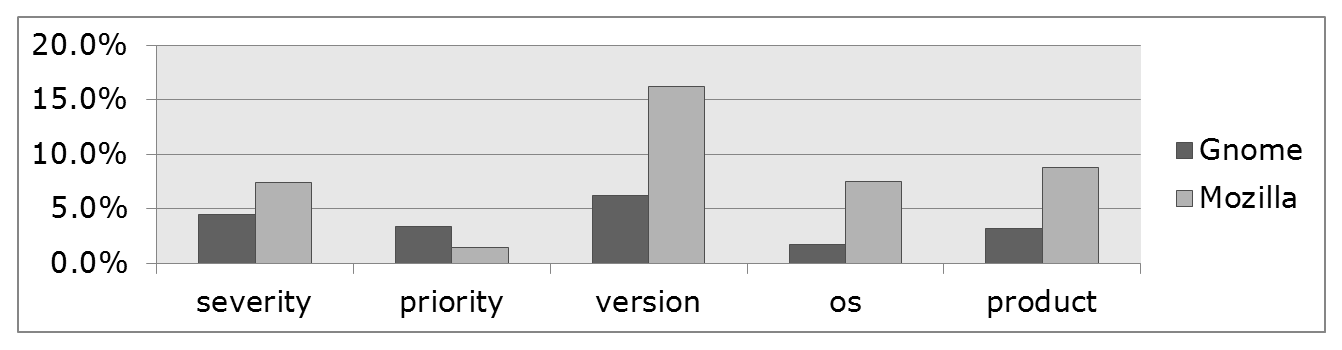
\epsfig{file=triage_practice.eps, width=6.8in,height=1.2in}
\end{centering}
\caption{Number of issues by triage task}
\label{fig:modification}
\end{figure*}
\end{comment}


\begin{table*}[ht]
\centering
\caption{The Number and Proportion of Issues with a Modified Attribute}\label{tab:modification}
\begin{tabular}{|r|r|r|r|r|r|r|}  \hline
  Project & Severity & Priority & Version & OS  & Product & Total Triaged Issues\\ \hline
  Gnome & 18K/4.4\% & 13K/3.3\% & 25K/6.2\% & 7K/1.7\% & 13K/3.2\% & 397K\\
  Mozilla & 18K/7.4\% & 4K/1.5\% & 40K/16.2\% & 19K/7.5\% & 22K/8.9\% & 249K\\
  \hline
\end{tabular}
\vspace{-0.1in}
\end{table*}

% following is in practice
% Maybe we should firstly show the result table, and give explanation to the differences
Table~\ref{tab:modification} shows the number and proportion of modifications to various
attributes of triaged issues in both communities. In particular, we see that
triagers modify Product, OS, Version and Severity in a larger fraction of
triaged issues for Mozilla and Priority in a larger fraction of triaged issues
for Gnome.

% we could draw some conclusion to common number here
% now we explain the differences
% need the % number in the paragraph? because we've put them in the figure
From the reviews and on-line documents and by inspecting a sample of
relevant issues, we found two reasons for these differences.  First,
the user base is different.  Mozilla has a much larger base of
users, thus an average user is likely to have less computer
expertise than an average Gnome user, e.g., ``Many bugs get
  marked Firefox when they are really bugs in the core engine.''
Such broad base of users also lowers the quality of reports and
requires triagers to add sufficient information to make them useful
for developers.

The second reason we found stems from the differences in community
policy.  For example, Mozilla Triage Guideline notes: ``don't change
  Priority field, which is for the
  developer''~\cite{mztriage}. This may partly explain why
Priority field is changed less in Mozilla.

% Triage involves filtering reported issues, filling information for
%  them, and assigning them to products.  Different project context
%  may lead to different triage practices affected by the type of
%  users and by community policies.  Both developers and
%  non-developer volunteers work on triage tasks.

% we've introduced we focus on triagers, do we still need the following paragraph?
\begin{comment}
Unlike code contributors, many triagers are
non-developer volunteers. For example, Gnome established a triage
team, Bug-Squad, to encourage volunteers who ``do not need any programming
knowledge'' to ``return something to the GNOME community if you
cannot program at all'' in order to ``make sure that major bugs do
not go unnoticed by
developers''~\footnotemark[2]. %{https://live.gnome.org/Bugsquad/}.
In this study we focus on triage done by non-developers, and investigate
their contributions to the community. The term $triager$ used in
later sections specifically refers to these contributors.
\end{comment}

\subsection{Impact of Triagers in Mozilla and Gnome}\label{ss:impact}
We evaluate triager's contribution by the number of modified issues
and the accuracy of the information they provide to developers.
Given that a triager may change several attributes of an issue, or
change the same attribute of an issue several times, we calculate
triager's contribution by the number of modified issues.  To measure
accuracy, we consider the fraction of activities without
``mistakes''. We also compare triagers' contribution to that of
developers'.

%In this section we investigate how triagers help by quantifying
%the amount and quality of their work. We investigate triagers'
%impact via the number of issues being filtered, modified and
%assigned and, the quality of the triage activities.
\begin{figure}[t]
\begin{centering}
\vspace{0.1in}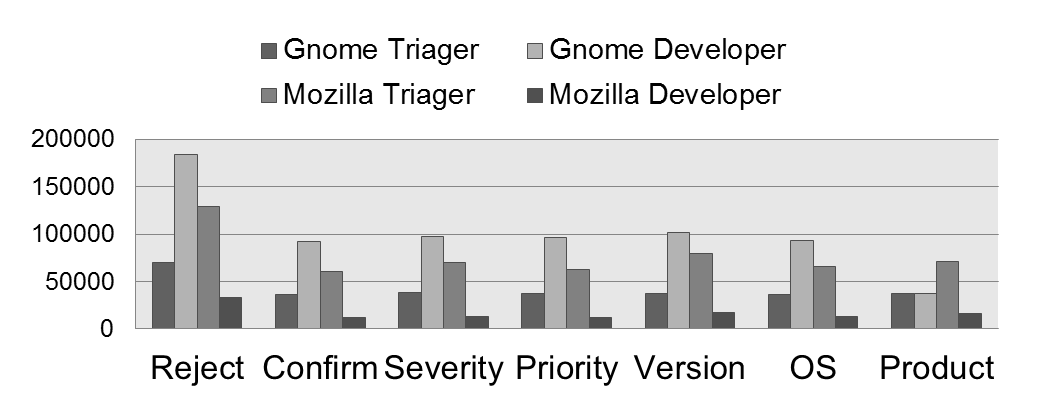
\epsfig{file=impact_amount.eps , width=3.4in,height=1.3in}
\end{centering}
\vspace{-0in}\caption{Number of Issues by Triage Task and Role}
\label{fig:impact_amount}
\end{figure}

\begin{figure}[t]
\begin{centering}
\vspace{-0.2in}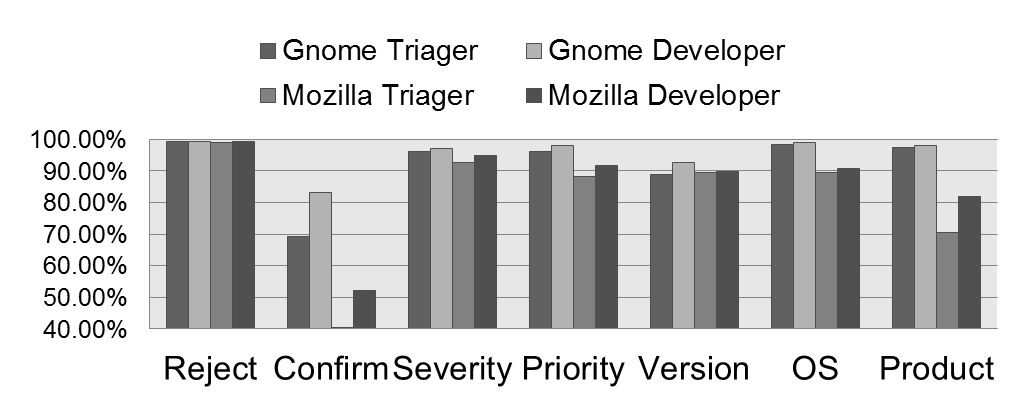
\epsfig{file=impact_quality.eps ,width=3.4in,height=1.3in}
\end{centering}
\vspace{-0in}\caption{Accuracy of Issues by Triage Task and Role}
\label{fig:impact_quality}
\vspace{-0.3in}
\end{figure}

Figure~\ref{fig:impact_amount} illustrates the number of issues for
different types of triage tasks and Figure~\ref{fig:impact_quality}
shows the quality of different types of triage tasks conducted by
triagers and developers in both communities.
Note Severity, Priority, Product, OS, and Version
represent the task of completing the corresponding
attribute.

\begin{comment}
\begin{table*}[ht]
\centering
\caption{Issues by triage task and role}\label{tab:field}
\begin{tabular}{|r|r|r|r|r|r|r|r|}
\hline
Project& Role & Rejected & Confirmed &  Severity & Priority & Version & OS & Product \\
  \hline
Gnome &  Triager & 71K & 36K & 38K & 37K & 38K & 36K & 37K  \\
  Developer & 184K & 92K & 97K & 96K & 102K& 93K & 98K  \\
  \hline
  \hline
Mozilla&   Triager & 116K & 54K & 172K & 170K & 177K & 171K & 64K \\
 & Developer & 33K & 11K & 45K & 44K & 48K & 45K & 16K \\
  \hline
\end{tabular}
\end{table*}
\end{comment}

Figures show that the biggest impact of triagers was on filtering reports.
In particular, the number of issues
filtered by triagers was $190K$ ($77$\% of all filtered issues) in Mozilla, and $106K$
($27$\% of all filtered issues) in Gnome. Meanwhile, triagers rejected issues
accurately: in both project, $99$\% of the rejections were correct, higher than
for any other type of task.



Triagers had the second largest impact on completing information for
newly reported issues, in particular, they completed attributes for
OS, Version, and Severity for a large number of issues and
accurately.  Gnome-1 commented on this finding: ``this
  information is meta data and can be easily asked for and corrected
  in one step.'' It suggests that completing the basic information
may be a good starting point for beginner triagers.

Figure~\ref{fig:impact_quality} shows that the triager product
assignments are often incorrect. It seems to be particularly
difficult in Mozilla: ``It can be an issue in the underlying stack instead
of the application, and finding the exact low-level library is hard for an
average triager.''


Table~\ref{tab:miscon} shows that
a large fraction of triager-confirmed issues are not fixed with
59\% and 30\% of issues confirmed by triagers were not fixed
(incorrectly confirmed) in Mozilla and Gnome respectively.


The largest fraction of such issues comes from duplicate reports.
The projects use some duplicate-detection technique, e.g., Mozilla
Crash Reports~\cite{mzcrep} and
Gnome Duplicate-finder, however, these techniques ``are not
perfect''~\cite{gntriage},
especially for those without stacktraces such as UI, enhancements or
translation problems.  Therefore, triager has to search through
existing reports, including the issues that are already fixed or
identified as duplicates.

Therefore, we expect that triagers may be most effective in reducing
developers' load by filtering irrelevant reports, and by filling in
missing information. But confirming issues and assigning them to the
correct products are not easy tasks for triagers.

\section{Validation and Limitations}\label{s:validation}
As mentioned earlier, we follow procedures described in~\cite{Changes07}
to ensure that we accurately interpret Bugzilla data and measures
derived from it.

In particular, we had to iterate to arrive at the method
we used to separate triagers from the other roles based on their
activity profiles. While it is relatively easy to identify developers
via their commits in the VCS, contributors may change their role
over time, with many triagers eventually contributing code (thus
becoming a developer). We, therefore, assigned a sequence ``(role,
time)'' of tuples to each individual based on the time when the role
was first assumed in the dataset. And we only considered a
contributor as a triager before she became a developer.  Meanwhile,
Reporters may conduct ``triage'' activities because anyone is
permitted to modify the issues they report.  We, therefore,
considered contributors to be triagers only if they triaged issues
reported by others.

A particularly vexing problem we faced was the measure of accuracy
for a triage activity. After many iterations and experimentation
with alternative measures we arrived at the presented heuristic even
though it has a number of drawbacks.  For example, typically
the severity of a NOTABUG issue is not considered to be important,
thus its final value may not be verified. We, therefore, did not
evaluate accuracy of activities with no subsequent activities for the same
issue, because the attributes modified by these activities may not
have had a chance to be looked at (and, thus, may not have been
verified).

We observed that some products changed their name. We, therefore, do
take it into account in calculating product assignment
accuracy. For example, if the final product value is B, but the
triager assigned the issue to product A.  We do not consider it to
be a mistake if the product A was renamed to B. To discover all instances of
product renaming we searched for inconsistencies in product names
data and validated these as instances of renaming by confirming via
documents describing the history of that product.
\vspace{-0.05in}

\section{Related Work}\label{s:related}
There has been a substantial amount of work on trying to understand
and help improve the issue/bug tracking practices.
%These investigations primarily focus on practices related to task
%assignment, (duplicate or similar) bug detectcoion, and the properties
%of bug reports.

``Who can fix this bug?'' is an important question
in bug triage needed to ``accurately'' assign developers to bug
reports.  For example, machine learning techniques~\cite{Anvik2006, Anvik2011},
and graph model based on Markov chains~\cite{Jeong2009},
were used to better assign developers to bug reports.
%Xuan et al.~\cite{xuan2012} considered leveraging the developer
%prioritization to assist the task of bug triage.

Detecting duplicate (or similar) reports is another
common topic, with studies attempting various ways to
compare the similarity of issue reports.  For example,
Natural Language Processing (NLP) techniques~\cite{Runeson07},
and NLP techniques plus execution information~\cite{Wang2008}
were used to suggest the most similar bug reports to the new bug report.

Bug fixing is an important topic with
a substantial amount of literature. Common questions include: which bugs get
fixed~\cite{ms10}? how long it takes to fix a bug~\cite{kim2006}?
%In particular, Guo et al.~\cite{ms10} performed an empirical study to characterize factors
%that affect which bugs get fixed in Windows Vista and Windows 7.
%Kim et al.~\cite{kim2006} studied the bug-fix time of files in ArgoUML and
%PostgreSQL by identifying when bugs are introduced and when they are fixed.
%Weiss et al.~\cite{Weiss07}  used the Lucene framework to search for similar,
%earlier reports and used their average time as a prediction for a new report.

Unlike prior work, this study focuses on understanding and quantifying
triagers' practice, in particular, what tasks a triager is involved with
and what value triagers may bring to the project.

\section{Conclusion}\label{s:conclusion}
We study the nature of triage and the impact of non-developer
triagers by analyzing the issue tracking practices in Gnome and Mozilla.

We found that the critical triage goals are to filter incoming
reports, fill incomplete information, and assign reports to
products. We also found some variations in triage practice between
the project that may be attributable to different policies and user
base. Our analysis shows that non-developer triagers make a substantial
contributions by filtering non-fixable issues and by filling basic
information, while confirming issues and assigning products
appear to be a difficult challenge for triagers.

We plan to use these results to investigate the reasons for the
difficulties triagers face in product assignement and in confirming
issues and we plan to develop tools to support such tasks.  In
particular, we plan to produce a tool that would help triage
practice by predicting the accuracy of all attributes in an issue
report and would suggest ways to correct it.  We hope that our work
would be worthy of the following quote from triager's guide:
``By following these techniques you will help the important bugs
  get fixed, as well as optimize precious developer time.''

\section{Acknowledgment}
Partial support by the National Natural Science Foundation of China
Grants 91118004, 61121063 and 61073016.

\balance

\bibliographystyle{IEEEtran}
\bibliography{all,audris}
\end{document}


